\documentclass[a4paper]{article}

\usepackage[english]{babel}
\usepackage[utf8]{inputenc}
\usepackage{amsmath}
\usepackage{multirow}
\usepackage{graphicx}
% \graphicspath{ {images/} }
%\usepackage[colorinlistoftodos]{todonotes}

\title{CS425A Project Report : P2P Video Streaming \\ Group 1}

\author{\hspace{0.1cm}Anubhav Bimbisariye  \hspace{1cm} Deepak Kumar \\
		Roll 11131  \hspace{3.0cm} Roll 12228\\
        \\
        \hspace{0.1cm}Siddhant Manocha \hspace{1.5cm} Pratik Somani\\
        Roll 12714 \hspace{3.0cm} Roll 11534\\
        }

\date {\today} 

\begin{document}

\maketitle

\begin{abstract}
% This is a Project report for our CS425A Course project on implementing Peer-to-peer live video streaming along with additional features.

We aim to wrap the browser's WebRTC implementation to provide an easy-to-use peer-to-peer live video streaming.The project is equipped with nothing but the room via which a peer can create a P2P media stream connection to a remote peer.

\end{abstract}

\section{Introduction}
Our project aims to build a robust system which will enable its users to create a live two way connection between them and stream each other's camera feed to the other user's browser. In this way we can ensure an efficient live peer-to-peer video streaming mechanism between the two nodes. 
% This functionality is similar to a live video chat among the participants, and so we require the transfer of video data to be smooth and of decent quality. 
In order to fulfill our objective, we build our project on node.js using express framework and socket.io which enable us to transfer data streams in real time.We also utilise getUserMedia API of HTML5 which grant web apps access to the camera and microphone without a plug-in and helps to enable high quality video and audio communication as part of WebRTC. \\
On one end, we have a node.js server node which bypasses the stream, and on the other end we have  clients connected to the server on common rooms.We access audio and video from the browser using getUserMedia API and sample the input into images and fixed size audio packets which are then transferred to the corresponding node at a fixed rate.
% On one end, we have a client setup a node.js server node, and on the other end we have another client connecting to this serverUsing this connection establishment, we can transfer the video feed to the corresponding nodes after periodic sampling of video data.
\section{Framework}
The project was built on the Ubuntu operating system using certain open-source modules and libraries.However the client can be used on any environment.The major components of the model are-
\begin{itemize}
\item Node.js
\item Socket.io
\item navigator.getUserMedia
\end{itemize} 
The project was built using the express framework of node.js and the streaming protocols in socket.io. Node.js is an asynchronous event driven framework, designed to build various network applications which are scalable in nature.Socket.io is used for real-time bidirectional event-based communication in network applications.The getUserMedia API is a feature of HTML5 which provides access to multimedia streams (video, audio, or both) from local devices.Developers can now access audio and video sources with a single function call, while users don’t need to install additional software.This provides live user media stream in real time which can be transferred from peer to peer.
\section{Methodology}
For clean and live peer-to-peer video streaming between two nodes, we need to ensure the following-
\begin{itemize}
\item We need to establish a reliable connection between the two nodes using socket.io
\item Ensuring smooth and robust data transfer between the two nodes for efficient real time video streaming without lag
\end{itemize}
In this project we use socket.io for conncection establishment and socket creations between the two nodes.After the connection establishment is complete, a suitable method for capturing video data on one end and transmitting it through the communication channel is needed. \\
In order to devise a suitable method for video streaming, we first sought to build live text messaging between the two peers, for if text messages could be sent in a streaming fashion from one node to the other, then using a similar mechanism, we can send video frames to and fro.\\
Once the simple chat client was built, we incorporated a method to capture frames as images using the computer's webcam at regular intervals, and then we send it in binary encoded format to the peer node, where it is decoded and rendered on HTML5 canvas.
\section{User Interface}
The user interface gives a form where users provide the username and the chat roomname as the input.Users are then connected to the given room and can communicate with any other peer connected to the same room.The video streaming interface consists of a small display window for the users' self feed,which is precisely the input captured by his camera and transmitted to the peer.A larger window displays the video stream of the peer connected to the same room.On the right side, a chat client is implemented. Users can type in their messages and send them like an ordinary chat.Microphone enabled machines can also send audio streams to the peer to facilitate audio chat.\\
Snapshots of the UI are included below.
\subsection{Snapshot} 

\begin{figure}[ht!]
\centering
\includegraphics[width=90mm]{images/im1.png}
\caption{Login Screen \label{overflow}}
\end{figure}

\begin{figure}[ht!]
\centering
\includegraphics[width=90mm]{images/im2.png}
\caption{Video Chat \label{overflow}}
\end{figure}

\begin{figure}[ht!]
\centering
\includegraphics[width=90mm]{images/im3.png}
\caption{Peer to Peer Communication \label{overflow}}
\end{figure}

\section{Working}
The process of live video streaming takes place as follows:
\begin{enumerate}
\item A machine running node.js starts the application, and creates a node.js server running at a specific port.It puts in a name to identify itself and a chatroom name to manage connection with other node.
\item Another machine starts the application and follows the same process, enters the chatroom name. If the chatroom name is being used by another machine, the two get connected and are able to transfer data to each other.

This creation of sockets and connections are supported by socket.io.\\
\item An instance of the application has two main events associated with it: \textit{emit} and \textit{listen}.

\textbf{Emit}: After every 33ms, we call appropriate functions to capture frames from the webcam feed, process them and send these captured images across the connection indicated by the chatroom.
\textbf{Listen(on)}: Whenever we receive data (ideally after ~33ms, but it depends on network connectivity), we process this data and display it on the screen using a canvas render.
\item Both the machines connected to a chatroom have these events. Since frames are sent every 33ms, rendering of consecutive frames appears to be like a video.
\item On the emit event, the frame being sent is displayed on the same machine too using the same rendering modules, so that user knows what is being transmitted.
\item One window on screen shows self camera feed on every emit event, and other window shows recieved feed on every 'on' event.
 
\end{enumerate}
 In this way we ensure video streaming by continuous sending of frames of the video from the sending end to the receiving end.
 
 Some other characteristics are:
 
\begin{itemize}
 \item \textbf{Webcam Processing}:
\textit{webcam-access.js} defines parameters such as resolution of video, functions to handle frame capture from the webcam, getting cam access permissions, etc.It also includes relevant code for capturing the audio stream from the microphone and the functions for encoding of the media stream.

\item \textbf{Frame encoding}:
Image is encoded in Base64-String format which is converted into binary format and sent over the socket.
\item \textbf{Movement Conscious Feed}:\\
To improve the quality of transmission and avoid long queues of untransferred frames,we came up with the solution to send video frames to the peer if the difference in the RMS value with the previous frame is atleast some minimum threshold value.This ensures that we only send frames which deviate largely from the previous frames.This reduces the load when user remains in static posture and increases the efficiency of transmission. 
% To prevent transmission when it might not be needed, there is a feature implemented to send feed only if the RMS value of the next frame differes by at least some minimum threshold value. This implies that frames are sent only when there is significant movement in the video feed.
This method increases the quality of the video and prevents lag among the video frames being sent from one end and those being received at the other end.
The disadvantage of this is that extremely slow and subtle movements are not picked up by the model. Also, the feed might result in a jerky video if the subject moves slowly to another position and then a fast movement takes place.However if the internet connection is good enough then we can disable this feature to enable normal transmission.
\end{itemize}
 \section{Additional Features}
We have incorporated several additional features to our P2P video-streaming model which work simultaneously with the video transfer and enhances the user-experience. 
\begin{itemize}

\item \textbf{Room functionality}: Socket.io enables the users to create rooms, using which each socket can be assigned to broadcast messages to a particular cluster or group. Using this feature in our model, two different nodes can connect to each other by joining the same room and running the application.This can also provide secured communication in case the rooms are password protected. After the connection establishment, two people (nodes) in the same room can send video streams from one end to the other without the intervention of any other user connected to the same server.
\item \textbf{Audio streaming}: We have incorporated a system which allows audio data to be transmitted from one client to the other, which occurs in parallel with the video streaming. This allows the users to communicate using both video and audio simultaneously, creating a video-chat like experience.
\item \textbf{Chat client}: Originally built as a prototype model to start the project, we have included a two-way chat client UI, which works in synchronization with the video and audio streaming. This enables the users to send text messages to each other, apart from the normal video chat.

\end{itemize}


\section{ Results}
We ran this application on two machines running Ubuntu connected by an Ethernet cable. The video stream obtained using ethernet cable was smooth and the video appeared stable. The quality of the video transmission decreased when the process ran over WiFi due to weaker internet connectivity between the nodes.

%%% INSERT IMAGES HERE 

% \includegraphics{im1}
% \includegraphics{im2}
% \includegraphics{im3}







\section{Conclusions} 
This application provides smooth peer-to-peer video streaming between two nodes, and allows the users to communicate with each other via video,audio or normal chat. The video stream performed better with the two machines connected by an ethernet cable, and the quality of the video decreased when connected over WiFi. The differences in video stream quality over WiFi, internet and LAN connection are noticeable.The stream of audio was satisfactory but had a lot of noice involved while capturing the audio from the microphone.
In terms of future work, there is scope for improvement in certain areas. In order to send high quality frames in an optimised fashion in our approach, an efficient compression method can be implemented to reduce the image size of each frame sent. The common compression like zip format were considered in the existing project and are not efficient enough to provide any significant improvement in terms of number of bits required to represent the compressed image.We can implement efficient vision based algorithms that use sparse encoding methods to represent the images that can be readily transferred over the Internet. Also, the audio streaming could be improved so as to provide more synchronised and smooth audio transmission.










%\bibliographystyle{plain}
%\bibliography{sample}

\end{document}
